\documentclass[11pt]{article}

% ------------------------------------------------------------------
%  Statistics Lab (52568) — Semester Summary
%  Group 12 — Shir, Omer & Ido
%  Compile with pdflatex or xelatex.
% ------------------------------------------------------------------

\usepackage[margin=1in]{geometry}
\usepackage{amsmath, amssymb}
\usepackage{booktabs}
\usepackage{array}
\usepackage{enumitem}
\usepackage{xcolor}
\usepackage{graphicx}
\usepackage{float}
\usepackage[colorlinks=true, linkcolor=blue!50!black, urlcolor=blue!50!black]{hyperref}
\usepackage{titlesec}
\usepackage{parskip}
\usepackage{caption}

\captionsetup{font=small, labelfont=bf, skip=4pt}
\titleformat{\section}{\normalfont\Large\bfseries\color{blue!30!black}}{\thesection}{1em}{}
\titleformat{\subsection}{\normalfont\large\bfseries}{\thesubsection}{1em}{}

\newcommand{\code}[1]{\texttt{#1}}
\graphicspath{{figs/}}

\title{\textbf{Statistics Lab (52568)\\[2pt]
\large Semester Summary: Genomic Coverage, GC Bias,\\
and Copy-Number Estimation}}
\author{Group 12 --- Shir Tsarfaty, Omer Sutovsky, Ido Ravid}
\date{Summer Semester 2026}

\begin{document}
\maketitle
\tableofcontents
\newpage

% ==================================================================
\section{The Big Picture: One Problem, Seven Labs}
% ==================================================================

\subsection{Biological motivation}

Our genetic information is encoded in DNA molecules arranged as chromosomes. In a
healthy human cell there are 46 chromosomes: 22 homologous pairs plus one sex-chromosome
pair (XX or XY). The double-helix consists of two parallel strands of nucleotides
(bases A, C, G, T) held together by complementary pairing: A$\leftrightarrow$T and
C$\leftrightarrow$G. When a cell divides, the double helix unzips and each strand
is used as a template to synthesize its complement, so each daughter cell receives an
identical copy.

\textbf{Copy number variation (CNV)} refers to regions where this copying process goes
wrong. A segment can be duplicated (\emph{copy-number gain}) or deleted
(\emph{copy-number loss}), changing the number of copies of that genomic region from
the normal 2. CNVs are part of normal human variation, but they are far more frequent
in cancer, where the machinery controlling cell division is damaged:
\begin{itemize}[leftmargin=*]
  \item \textbf{Down syndrome} (trisomy 21) is caused by a third copy of chromosome 21,
    disrupting developmental balance.
  \item In \textbf{tumors}, copy-number gains of growth-promoting genes can drive
    uncontrolled proliferation. A 2005 study found that a growth hormone gene was
    amplified in the majority of nine tumor biopsies examined.
\end{itemize}
Detecting CNVs is therefore a clinically important problem. We measure them
indirectly through \textbf{sequencing coverage}.

\subsection{High-throughput DNA sequencing}

Next-generation sequencing (NGS, e.g.\ Illumina/Solexa) allows millions of short DNA
fragments to be read in a single run. The pipeline has three stages:
\begin{enumerate}[leftmargin=*]
  \item \textbf{Library preparation}: genomic DNA is fragmented into pieces of roughly
    uniform size and \emph{amplified by PCR} (copies made so there is enough material
    to sequence).
  \item \textbf{Sequencing}: each fragment is immobilized, copied base-by-base with
    fluorescently labelled nucleotides, and the color signal is read --- yielding a
    short \emph{read} of $\sim$70--100 bases from each end. The output is a FASTQ file
    with read sequences and quality scores.
  \item \textbf{Alignment (mapping)}: reads are aligned back to a reference genome
    (we use \code{hg18}, a consensus built by the Human Genome Project, 2000) using
    fast hash-based algorithms. The output is a SAM/BAM file storing the
    chromosomal location and length of each mapped fragment.
\end{enumerate}
We work with a filtered version of this output: a \code{.forward} file containing
\code{(Chromosome, Location, Length)} for one paired-read direction on chromosome~1.
Our patient is \code{TCGA-13-0723}, with a healthy tissue sample
(\code{-10B}) and a paired tumor sample (\code{-01A}).

\textbf{Coverage as a proxy for copy number.} The number of reads mapping to a region
is proportional to the number of DNA copies of that region in the sample: if a segment
is duplicated (4 copies instead of 2), it should on average produce twice as many reads.
For a single sample:
\[
  \frac{\text{reads at region}}{\text{reads at typical region}} \;\approx\;
  \frac{\text{copy number}}{2}.
\]
For two samples (tumor vs.\ normal), the ratio of read counts at a locus is proportional
to their copy-number ratio, assuming otherwise uniform coverage. The central difficulty
--- and the theme of the entire course --- is that coverage is \emph{not} uniform:
it is systematically distorted by the local GC content of the DNA sequence, a bias
introduced largely by the PCR step.

\subsection{The semester arc}

\begin{center}
\begin{tabular}{@{}clp{9.5cm}@{}}
\toprule
\textbf{Lab} & \textbf{Topic} & \textbf{What it adds} \\
\midrule
1 & Base composition & Describe the raw sequence; see Chargaff pairing; find high-GC region \\
2 & Coverage computation & Efficient read-counting; chromosome-wide coverage map; distribution \\
3 & Poisson assessment & Test the uniform model; discover overdispersion; find GC as the cause \\
4 & Spline regression & Model $f(\text{gc})$; residual analysis; learning curves \\
5 & GC analysis (AI-first) & G vs.\ C vs.\ G+C; spatial consistency; bin size; Poisson GLM \\
6 & Copy-number estimation & Plug-in estimator; variance decomposition; noise models \\
7 & Tumor vs.\ healthy & Two-sample comparison; aggregative bin-size selection \\
8 & GC correction review & (covered within Lab 9 analysis) \\
9 & Anomaly detection & Hypothesis testing; empirical null; FDR; CNV segmentation \\
\bottomrule
\end{tabular}
\end{center}

% ==================================================================
\section{Part I --- What We Learned}
% ==================================================================

\subsection{From reads to coverage}

The first computational lesson was that \emph{correctness and speed are separate
concerns}: always start from a slow version you trust, then optimize. Counting reads
per base can be done naively (loop over every base, scan for matching reads) or
efficiently with R's vectorized \code{tabulate()} function, which exploits the fact that
read locations are already sorted. Figure~\ref{fig:benchmark} shows the performance
difference over 100 random 1-Mb windows.

\begin{figure}[H]
  \centering
  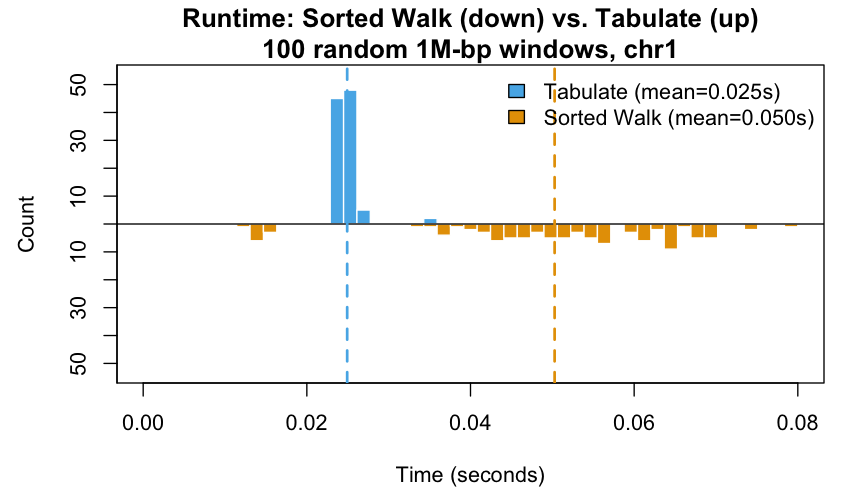
\includegraphics[width=0.72\textwidth]{fig_lab2_benchmark}
  \caption{\textbf{Lab 2 --- Algorithm benchmark.} Back-to-back histogram of runtimes
  over 100 random 1-Mb windows. \texttt{tabulate} (blue, up) averages 0.025 s;
  sorted walk (orange, down) averages 0.054 s --- more than twice as slow.}
  \label{fig:benchmark}
\end{figure}

\textbf{Binning.} Base-level coverage is extremely sparse (most bases have 0 or 1 read).
We aggregate reads into \emph{bins} of width $b$, so $Y_k = \sum_{\text{bases in bin}} Y_i$
is the working unit for all subsequent modelling. Bin size is a genuine modelling
choice with real tradeoffs (§\ref{sec:binsize}).

\subsection{The uniform Poisson model and its assumptions}
\label{sec:poisson}

The simplest model imagines reads landing like raindrops: each of the $J$ fragments
independently picks a start base, uniformly at random over the $I$ bases. This rests
on three explicit assumptions:
\begin{enumerate}[leftmargin=*]
  \item \textbf{Identical distribution} --- every fragment has the same landing
        probabilities.
  \item \textbf{Uniformity} --- $p_i = 1/I$ for all bases $i$.
  \item \textbf{Independence} --- fragments land independently.
\end{enumerate}
Under (1)+(3), $Y_i \sim \text{Binomial}(J, p_i)$. Adding (2) and the Poisson
approximation (large $J$, tiny $1/I$):
\[
  Y_i \;\sim\; \text{Poisson}(\lambda), \qquad \lambda = J/I .
\]
Because independent Poissons add, a bin satisfies $Y_k \sim \text{Poisson}(\lambda_k)$.
The defining testable property:
\[
  \mathbb{E}[Y] = \mathrm{Var}[Y] = \lambda
  \quad\Longrightarrow\quad
  \text{VMR} = \frac{\mathrm{Var}[Y]}{\mathbb{E}[Y]} = 1 .
\]
SD grows like $\sqrt{\lambda}$, so relative noise shrinks as bins grow --- a first
taste of the bias--variance tradeoff.

\subsection{Why the uniform model fails: overdispersion and the variance decomposition}

Real coverage is heavily \textbf{overdispersed}: VMR $\approx 14.7$ rather than 1.
The theoretical tool that explains \emph{why} is the \textbf{law of total variance},
applied to the natural two-level structure of our data.

\paragraph{The two-level model.}
We are \emph{not} claiming all bins share a single rate $\lambda$. The more honest
description is that each bin $k$ has its own rate:
\[
  Y_k \;\sim\; \text{Poisson}(\lambda_k),
\]
where $\lambda_k$ varies across the genome (driven by local sequence properties we
have not yet modeled). Each bin still satisfies the Poisson property
\emph{conditional on its own rate}:
\[
  \mathbb{E}[Y_k \mid \lambda_k] = \lambda_k, \qquad
  \mathrm{Var}(Y_k \mid \lambda_k) = \lambda_k.
\]
The question is: what is the \emph{marginal} variance of $Y_k$ when we also account
for the variation of $\lambda_k$ across bins?

\paragraph{The law of total variance.}
For any two random variables $Y$ and $X$:
\[
  \mathrm{Var}(Y) \;=\;
  \underbrace{\mathbb{E}\bigl[\mathrm{Var}(Y \mid X)\bigr]}_{\text{average within-group variance}}
  \;+\;
  \underbrace{\mathrm{Var}\bigl(\mathbb{E}[Y \mid X]\bigr)}_{\text{variance of group means}}.
\]
This is an exact identity --- no approximation or model assumption beyond the
existence of these moments. Setting $Y = Y_k$ and $X = \lambda_k$:
\[
  \mathrm{Var}(Y_k) \;=\;
  \mathbb{E}\bigl[\mathrm{Var}(Y_k \mid \lambda_k)\bigr]
  \;+\;
  \mathrm{Var}\bigl(\mathbb{E}[Y_k \mid \lambda_k]\bigr).
\]
Substituting the two Poisson identities:
\[
  \boxed{\mathrm{Var}(Y_k) \;=\;
  \underbrace{\mathbb{E}[\lambda_k]}_{\text{Poisson term (within-bin noise)}}
  \;+\;
  \underbrace{\mathrm{Var}(\lambda_k)}_{\text{rate variation (between-bin heterogeneity)}}}
\]
Writing this empirically over the $K$ observed bins (replacing population moments with
sample averages):
\[
  \mathrm{Var}(Y_k) \;\approx\;
  \bar\lambda \;+\; \frac{1}{K}\sum_{k=1}^K (\lambda_k - \bar\lambda)^2,
  \qquad \bar\lambda = \tfrac{1}{K}\textstyle\sum_k \lambda_k.
\]

\paragraph{Why VMR $= 1$ characterizes the uniform model.}
Dividing both sides by the mean:
\[
  \text{VMR} \;=\; \frac{\mathrm{Var}(Y_k)}{\mathbb{E}[Y_k]}
  \;=\; 1 \;+\; \frac{\mathrm{Var}(\lambda_k)}{\bar\lambda}.
\]
The VMR equals 1 \textbf{if and only if} all rates $\lambda_k$ are identical --- which
is exactly the uniform Poisson assumption. Any spatial heterogeneity in rates
pushes VMR above 1. Our observed VMR $\approx 14.7$ means:
\[
  \mathrm{Var}(\lambda_k) \;\approx\; 13.7 \cdot \bar\lambda,
\]
i.e.\ the rate-variation term is roughly 14$\times$ larger than the Poisson noise.

\paragraph{Why the rate-variation term is so large.}
One might expect that summing 5000 bases into a bin would average out rate
fluctuations (a central-limit argument). But this only works if neighboring bases
have \emph{independent} rates. In reality, nearby bases have similar GC content, so
their $\lambda$ values are positively correlated. When correlated quantities are
summed, variance does not shrink --- the rate variation persists at the bin scale.
This is exactly what GC content creates: spatially structured, persistent rate
heterogeneity that does not wash out under aggregation.

\paragraph{Summary of the terms.}
\begin{center}
\begin{tabular}{@{}lll@{}}
\toprule
\textbf{Term} & \textbf{Interpretation} & \textbf{Vanishes when\ldots} \\
\midrule
$\bar\lambda$ & Irreducible Poisson sampling noise & Never ($\lambda > 0$) \\
$\mathrm{Var}(\lambda_k)$ & Rate heterogeneity across the genome & All $\lambda_k$ are equal (uniform model) \\
\bottomrule
\end{tabular}
\end{center}

This decomposition is the conceptual engine of the semester: the course is about
\emph{modeling the second term} (via GC content) and removing it, so that coverage
reflects copy number (a biological signal) rather than sequencing bias.

Figure~\ref{fig:poisson} shows the observed vs.\ Poisson distribution (Lab~3), and
Figure~\ref{fig:gc_scatter} shows the GC--coverage scatter that explains the
discrepancy.

\begin{figure}[H]
  \centering
  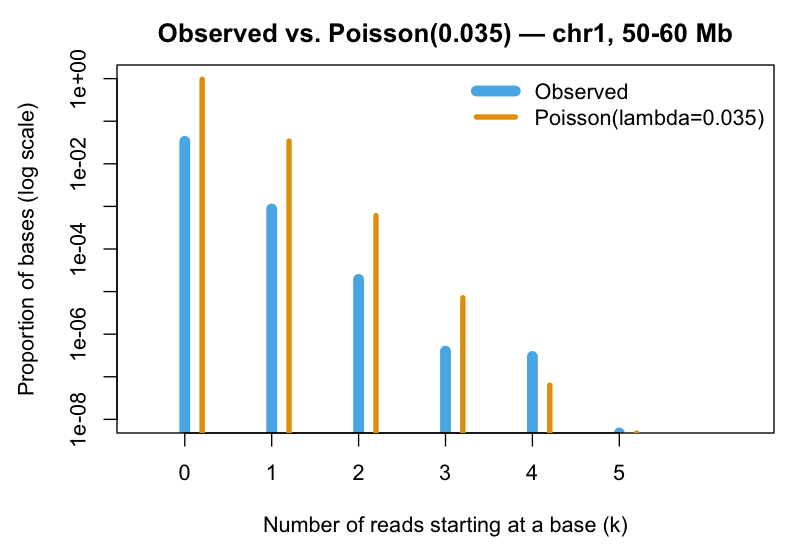
\includegraphics[width=0.68\textwidth]{fig_lab3_poisson}
  \caption{\textbf{Lab 3 --- Observed vs.\ Poisson distribution.}
  Blue: observed proportions of bases with $k$ reads (log scale).
  Orange: Poisson($\lambda=0.035$) prediction. The observed distribution is
  clearly less left-skewed and more right-skewed than Poisson, confirming the model fails.}
  \label{fig:poisson}
\end{figure}

\begin{figure}[H]
  \centering
  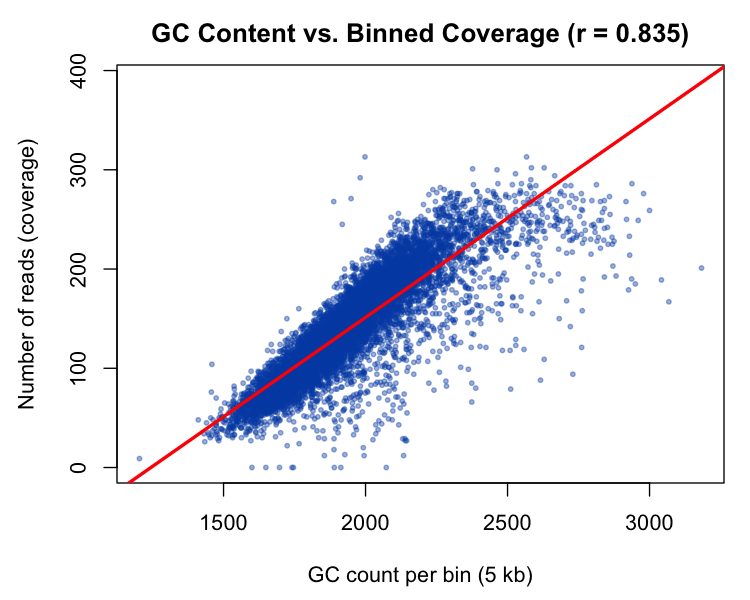
\includegraphics[width=0.60\textwidth]{fig_lab3_gc_scatter}
  \caption{\textbf{Lab 3 --- GC content vs.\ binned coverage (50--100 Mb, 5 kb bins).}
  Strong positive linear trend ($r \approx 0.84$, red line). GC-rich bins attract
  systematically more reads, violating the uniformity assumption.}
  \label{fig:gc_scatter}
\end{figure}

\subsection{The GC-content bias and the Benjamini \& Speed (2012) paper}
\label{sec:gc}

This is the central phenomenon of the course, and of our professor's own paper:
\textbf{Benjamini \& Speed (2012), ``Summarizing and correcting the GC content bias
in high-throughput sequencing,'' \textit{Nucleic Acids Research} 40(10):e72.}

Key findings from the paper:
\begin{itemize}[leftmargin=*]
  \item The relationship is \textbf{unimodal}: both GC-rich \emph{and} AT-rich
    fragments are underrepresented; coverage peaks at intermediate GC ($\approx$50\%).
    (At our 50--100~Mb binned scale we see mostly the rising left arm, but the spline
    captures the curvature.)
  \item The GC content of the \textbf{entire fragment} (not just the sequenced read)
    drives the bias most strongly --- evidence that \textbf{PCR amplification}, not
    sequencing chemistry, is the main cause.
  \item After correcting for GC, copy-number gains hidden by the bias become visible.
    The paper demonstrates recovery of a CN gain on chromosome~2 in tumor data.
\end{itemize}
The course implements this correction step by step, using the same conceptual
framework: model coverage as $a_k \cdot f(\text{gc}_k)$, estimate $f$, divide it out.

\subsection{The full-chromosome view}

\begin{figure}[H]
  \centering
  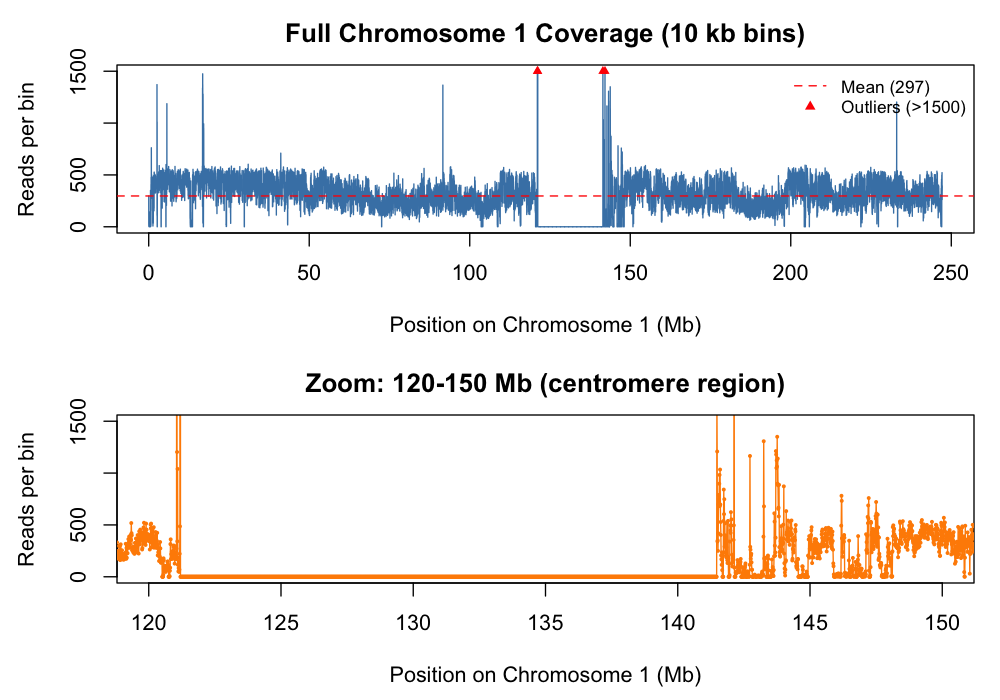
\includegraphics[width=0.88\textwidth]{fig_lab2_coverage}
  \caption{\textbf{Lab 2 --- Full chromosome coverage and centromere zoom.}
  \textit{Top:} Coverage across all of chromosome~1 (10 kb bins). The dashed red line
  is the mean. Black vertical lines mark the zoom region. Red triangles mark outlier
  bins clipped at 1500 reads. Note the coverage gap at $\sim$120--130 Mb (centromere)
  and extreme spikes at $\sim$130--145 Mb (likely duplicated segments).
  \textit{Bottom:} Zoom-in on 120--150 Mb showing the centromere gap clearly.}
  \label{fig:coverage}
\end{figure}

\subsection{Regression: linear, then non-parametric (splines)}

We first modelled $f$ linearly via \code{lm}: $Y_k = \beta_0 + \beta_1\,\text{gc}_k + \epsilon_k$.
This introduced the regression toolkit: coefficients and standard errors, residual
plots, RMSE, the danger of outliers, and the formula
$\hat\beta_1 = \widehat{\mathrm{Cov}}(\text{gc},Y)/\widehat{\mathrm{Var}}(\text{gc})$.

The true relationship is curved (Figure~\ref{fig:splines}), motivating
\textbf{spline regression}. The key ideas, built up from first principles in lecture:
\begin{itemize}[leftmargin=*]
  \item Partition the predictor range at \textbf{knots}; fit a polynomial in each piece.
  \item Enforce smoothness at knots: a \textbf{cubic regression spline} keeps the function
    and its first two derivatives continuous, using truncated-power basis functions
    $f_d(x,t)=(x-t)^d\cdot\mathbf{1}\{x>t\}$.
  \item B-splines (\code{bs()} in R) give the same fit with a better-conditioned,
    locally supported basis.
  \item Modelling choices: \textbf{knot count/placement} and \textbf{degree}.
    More knots $\Rightarrow$ more flexibility; higher degree $\Rightarrow$ smoother curves.
  \item Despite the non-parametric spirit, the model is fit by ordinary OLS on the
    basis columns --- so all standard regression tools (residuals, $R^2$, AIC) apply.
\end{itemize}

\begin{figure}[H]
  \centering
  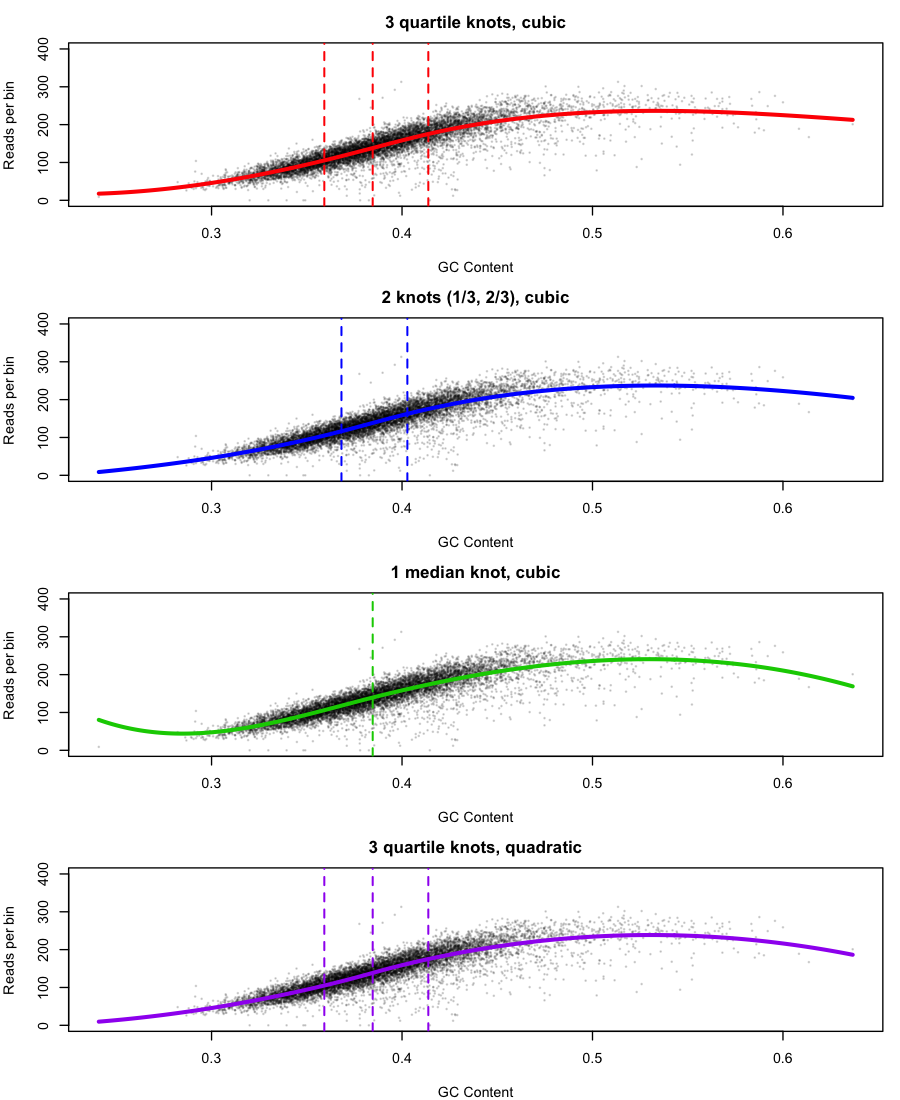
\includegraphics[width=0.80\textwidth]{fig_lab4_splines}
  \caption{\textbf{Lab 4 --- Four B-spline models for GC--coverage.}
  Each panel shows GC content (x) vs.\ reads per 5 kb bin (y, gray points) with the
  fitted spline (colored line) and knot positions (dashed verticals). All four
  models capture the main trend similarly; the models diverge in the high-GC tail
  where data are sparse. $R^2 \approx 0.75$ for all candidates.}
  \label{fig:splines}
\end{figure}

\subsection{Model selection, generalization, and the bias--variance tradeoff}
\label{sec:binsize}

Flexible models risk overfitting, so we judge them \textbf{out-of-sample}:
train/validation/test splits (\code{set.seed} for reproducibility),
\textbf{learning curves} (validation RMSE vs.\ training-set size), and robust
metrics alongside RMSE (median, IQR, median absolute error).

\begin{figure}[H]
  \centering
  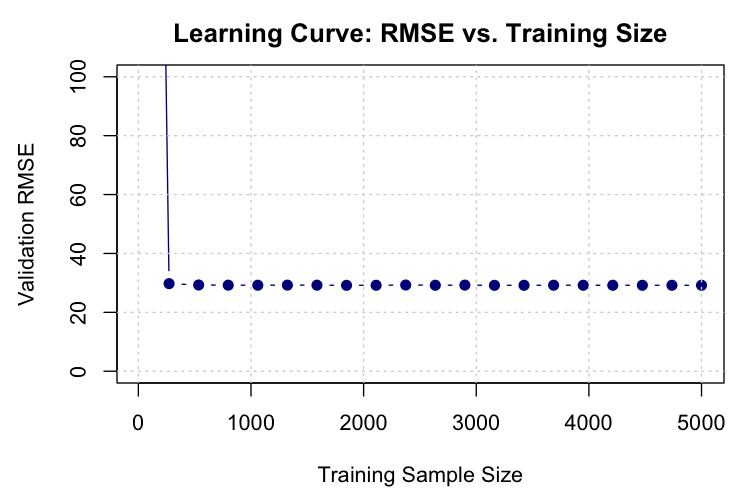
\includegraphics[width=0.68\textwidth]{fig_lab4_learning}
  \caption{\textbf{Lab 4 --- Learning curve.}
  Validation RMSE as a function of training sample size. RMSE drops sharply from
  $\sim$100 at $n=10$ and plateaus near 30 by $\sim$500 samples, showing the GC trend
  is learnable with little data.}
  \label{fig:learning}
\end{figure}

The \textbf{bias--variance tradeoff} appears most clearly in \textbf{bin size}.
Larger bins average out per-base Poisson noise (lower variance) but blur the local
GC signal and smear genomic features (higher bias). Figure~\ref{fig:binsize} shows
the marginal $R^2$ gain from increasing bin size. The statistical \emph{elbow} falls
near 5 kb; combined with the scale of biological features (genes 10--100 kb, CpG
islands 0.5--2 kb), 5 kb is a principled choice.

\begin{figure}[H]
  \centering
  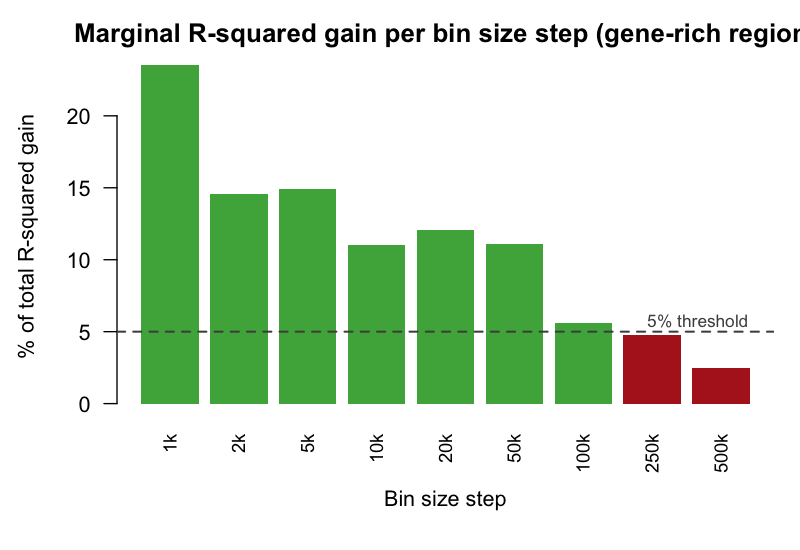
\includegraphics[width=0.75\textwidth]{fig_lab5_binsize}
  \caption{\textbf{Lab 5 --- Marginal $R^2$ gain per bin-size step (gene-rich region).}
  Green bars contribute $\geq$5\% of the total gain; red bars represent diminishing
  returns below the threshold. The elbow falls at $\sim$5 kb: beyond this, more
  aggregation costs spatial resolution without meaningfully improving the model.}
  \label{fig:binsize}
\end{figure}

\subsection{GC-skew and why G+C beats either alone}

\begin{figure}[H]
  \centering
  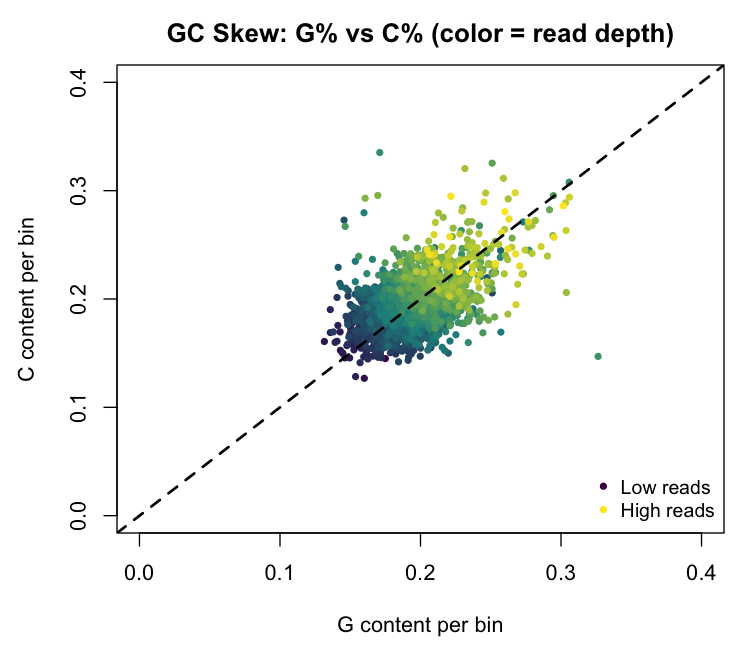
\includegraphics[width=0.62\textwidth]{fig_lab5_gcskew}
  \caption{\textbf{Lab 5a --- GC skew: G\% vs C\% per bin, color = read depth.}
  The cloud follows the Chargaff diagonal (G\% $\approx$ C\% globally), but fans out
  at higher GC values. High-GC bins (yellow = high reads) spread away from the
  diagonal due to transcription-coupled strand asymmetry in gene-rich regions. This
  means C carries independent signal precisely where coverage is highest --- hence
  \texttt{\textasciitilde G+C} outperforms \texttt{\textasciitilde G} alone by $\approx$0.17 in $R^2$.}
  \label{fig:gcskew}
\end{figure}

\subsection{Spatial consistency of the GC--coverage relationship}

\begin{figure}[H]
  \centering
  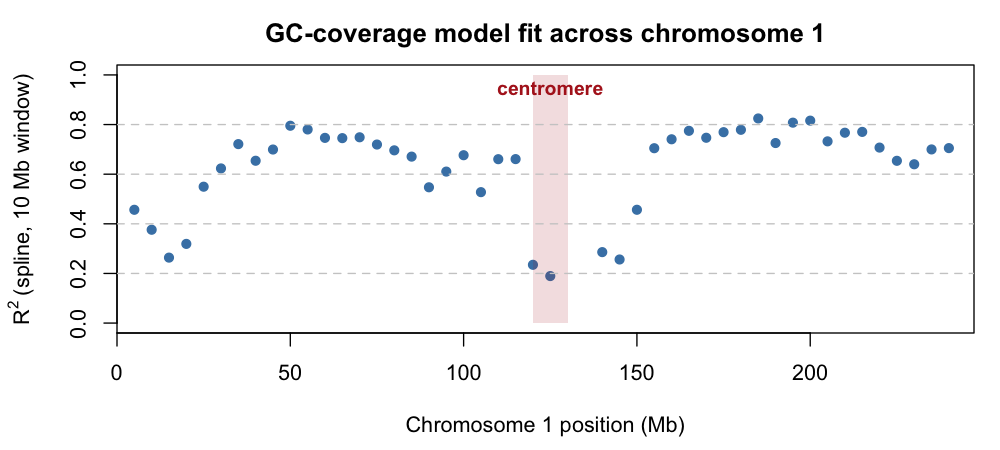
\includegraphics[width=0.85\textwidth]{fig_lab5_spatial}
  \caption{\textbf{Lab 5b --- Spatial $R^2$ profile across chromosome 1.}
  Each dot is the spline model $R^2$ for a 10 Mb window. Gene-rich regions reach
  $R^2 \approx 0.7$; the centromere ($\sim$120--130 Mb, shaded red) drops to $\approx 0.3$.
  The relationship is not spatially uniform --- per-region fitting is justified.}
  \label{fig:spatial}
\end{figure}

\subsection{Poisson GLM and quasi-Poisson}

Because the response is a count, the natural regression is a \textbf{generalized
linear model} with log link: $\log\mathbb{E}[Y_k] = \beta_0 + \beta_1\,\text{gc}_k$.
Plain Poisson GLM forces $\mathrm{Var}(Y)=\mathbb{E}[Y]$, which we know is violated.
\textbf{Quasi-Poisson} relaxes this to $\mathrm{Var}(Y)=\phi\,\mathbb{E}[Y]$ and
estimates dispersion $\phi$ directly. The two give nearly identical fitted means but
different uncertainty estimates. The residual $\phi\approx 14$ after including GC
confirms substantial overdispersion remains --- GC explains part but not all of the
extra variance.

\subsection{The copy-number estimation model}
\label{sec:cn}

Everything converges here. The generative model is:
\[
  Y_k \;\sim\; \text{Poisson}(\lambda_k), \qquad
  \lambda_k \;=\; a_k \cdot f(\text{gc}_k) \;+\; \epsilon_k,
\]
with identifiability constraints: $\mathrm{med}_k\{a_k\}=1$,
$\mathbb{E}_k[f(\text{gc}_k)]=1$, $\mathbb{E}[\epsilon_k]=0$.

Solving for $a_k$ and substituting our spline estimate $\hat f$ gives the
\textbf{plug-in estimator}:
\[
  \hat a_k \;=\; \frac{y_k}{\hat f(\text{gc}_k)} \cdot \hat M,
  \qquad
  \hat M = \frac{1}{\mathrm{med}_k\!\left\{\dfrac{y_k}{\hat f(\text{gc}_k)}\right\}},
\]
i.e.\ \emph{divide out the GC effect, then renormalize} so the median estimate is
exactly 1. Normal genomes should concentrate around 1; departures flag CN events.

\subsection{Variance decomposition of the estimator}

To leading order,
$\mathrm{Var}(\hat a_k) \approx \bigl[\lambda_k + \sigma^2\bigr]/f(\text{gc}_k)^2$,
where the first term is irreducible Poisson sampling noise and the second is technical
$\epsilon$ noise ($\sigma^2$ estimated from spline residuals, no normality assumed).
Their relative shares tell us whether \textbf{more reads} (shrinks the Poisson term)
or a \textbf{better technical model} (shrinks the $\epsilon$ term) is the path to
improvement.

\subsection{The two-sample noise decomposition (Yuval's theory note)}

Yuval's second copy-number note provides a richer two-sample model. The noise in a single
sample is decomposed into a \textbf{shared component} $\gamma_k$ (same in both tumor and
healthy, e.g.\ local mappability, chromatin structure) and \textbf{sample-specific} components
$\delta_k^T$, $\delta_k^N$:
\[
  Y_k^T = a_k \cdot f^T(\text{gc}_k) \cdot \gamma_k \cdot \delta_k^T + \eta^T_{k},\qquad
  Y_k^N = f^N(\text{gc}_k) \cdot \gamma_k \cdot \delta_k^N + \eta^N_{k} .
\]
The two-sample estimator
\[
  \hat a_k^{(2)} = \frac{Y_k^T / \hat f^T(\text{gc}_k) + c}{Y_k^N / \hat f^N(\text{gc}_k) + c}
  \;\approx\; a_k \cdot \frac{\delta_k^T}{\delta_k^N}
\]
cancels the shared component $\gamma_k$ entirely --- what remains is only the ratio of the
sample-specific noises $\delta_k^T/\delta_k^N$. This is the key advantage over single-sample
correction: if the dominant technical variation is shared (mappability, GC curves of the same shape), the two-sample ratio is much cleaner than either sample alone.

The stabilized single-sample estimator $\hat a_k^{(1*)} = (Y_k+c)/(\hat f + c)$ trades a small
increase in bias (for bins where $a_k\neq 1$) for reduced variance at low-coverage bins.

\subsection{Additive vs.\ multiplicative noise}

Should the noise be \textbf{additive} ($\lambda_k = a_k f + \epsilon$, fixed-size
offset) or \textbf{multiplicative} ($\lambda_k = a_k f \cdot \eta$,
$\eta\sim N(1,\gamma^2)$, noise scaling with signal)? Biologically, the multiplicative
form is more plausible: PCR amplifies errors in proportion to the amount of DNA, so
larger expected coverage carries larger absolute fluctuations --- consistent with the
heteroscedasticity we observed (residual spread grows with GC/coverage).

\subsection{Two-sample comparison: tumor vs.\ healthy}

With a healthy sample as baseline (copy number $\approx1$ everywhere) and a paired
tumor sample, the GC correction is fit \emph{separately per sample} (the bias
function differs between libraries). After per-sample correction and median
normalization, bins where tumor and healthy CN diverge are candidate CN events.
This is exactly the paper's demonstration: a copy-number gain hidden by GC bias
becomes visible after correction.

% ==================================================================
\section{Part II --- Our Lab Results}
% ==================================================================

\subsection{Lab 1 --- Base composition of chromosome 1}

We counted A/C/G/T in 1000-bp cells over 50--70~Mb. Running medians ($k=201$,
Figure~\ref{fig:runmed}) confirmed \textbf{Chargaff pairing}: A and T track each
other, as do C and G. Pair scatter plots (Figure~\ref{fig:scatter}) showed the
strongest positive correlations for A--T and C--G. We flagged a
\textbf{high-GC anomaly at cells $\sim$3000--5500 ($\approx$53--55.5 Mb)}, visible
as the shaded region in the lab.

\begin{figure}[H]
  \centering
  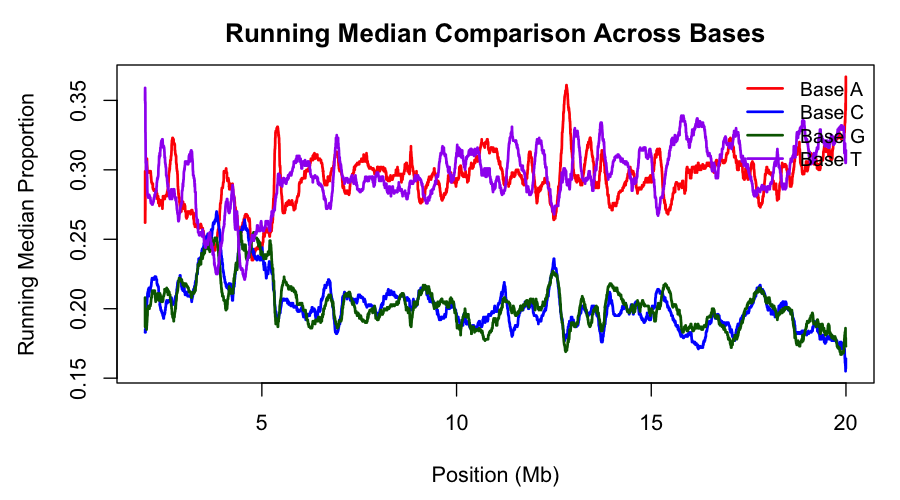
\includegraphics[width=0.82\textwidth]{fig_lab1_runmed}
  \caption{\textbf{Lab 1 --- Running median comparison across bases.}
  Smoothed proportions of A (red), C (blue), G (dark green), and T (purple) along
  the chromosome. A$\approx$T and C$\approx$G throughout, confirming Chargaff's rule.
  C and G are systematically lower, consistent with a slight AT bias in the analyzed region.}
  \label{fig:runmed}
\end{figure}

\begin{figure}[H]
  \centering
  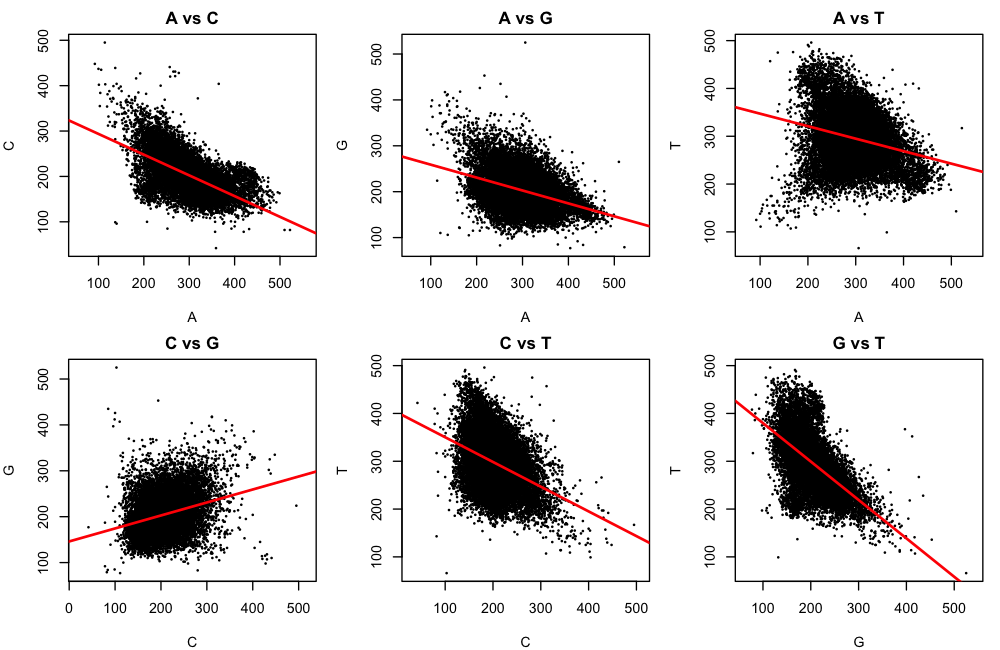
\includegraphics[width=0.82\textwidth]{fig_lab1_scatter}
  \caption{\textbf{Lab 1 --- Pairwise base-count scatter plots.}
  Each point is one 1000-bp cell. The A--T and C--G pairs (anti-diagonal entries)
  show the clearest positive correlations with red regression lines. The C--G cloud
  clusters near the origin (lower absolute counts) but has striking upper-right
  outliers corresponding to the high-GC region at 53--55.5 Mb.}
  \label{fig:scatter}
\end{figure}

\subsection{Lab 2 --- Coverage computation and chromosome-wide distribution}

We implemented and benchmarked two coverage algorithms (Figure~\ref{fig:benchmark}).
Full-chromosome binned coverage (10 kb bins, Figure~\ref{fig:coverage}) revealed:
\begin{itemize}[leftmargin=*]
  \item \textbf{Centromere gap} at $\sim$120--130~Mb: coverage collapses to near zero
    (low-complexity, poorly-mappable repetitive sequence).
  \item \textbf{Outlier spikes} at $\sim$130--145~Mb: extreme coverage likely caused
    by reads mapping to duplicated segments.
  \item \textbf{Elevated coverage} at 0--30~Mb: also suggestive of copy-number
    variation or mappability artefacts.
\end{itemize}
A Normal fit to the binned coverage distribution was poor: heavy left tail, missing
right tail, too flat in the middle.

\subsection{Lab 3 --- Testing the uniform Poisson model}

Region 50--60~Mb, bins of 5000~bp. Results:
\begin{itemize}[leftmargin=*]
  \item Base-level mean coverage $\lambda \approx \mathbf{0.036}$ reads/base.
  \item Observed vs.\ Poisson mismatch (Figure~\ref{fig:poisson}): distribution is
    less left-skewed and more right-skewed than Poisson.
  \item Binned \textbf{VMR} $\approx \mathbf{14.7}$ (Poisson predicts 1); IQR
    $\approx 5\times$ the Poisson expectation. Decisive overdispersion.
  \item GC--coverage correlation $\mathbf{r \approx 0.84}$ over 50--100~Mb
    (Figure~\ref{fig:gc_scatter}), consistent with the Dohm et al.\ paper and our
    professor's work. This explains the Poisson failure: coverage is driven by
    GC, not a uniform process.
\end{itemize}

\subsection{Lab 4 --- Spline regression for $f(\text{gc})$}

Region 50--100~Mb, 5000-bp bins. Four B-spline candidates varying knot count (1--3)
and degree (2--3); all performed similarly (Figure~\ref{fig:splines}).
Key findings:
\begin{itemize}[leftmargin=*]
  \item $R^2$ capped at $\approx \mathbf{0.75}$; knot count mattered more than degree.
  \item Residual-SD ratio (high-GC quartile / low-GC quartile) $\approx \mathbf{2.25}$
    $\Rightarrow$ \textbf{heteroscedasticity}: error variance grows with coverage.
  \item Learning curve (Figure~\ref{fig:learning}): RMSE drops sharply and plateaus
    after $\sim$500 training bins --- the GC trend is learnable from little data.
\end{itemize}

\subsection{Lab 5 --- The GC relationship in depth (AI-first)}

\begin{description}[leftmargin=0pt]
  \item[(a) G vs.\ C vs.\ G+C:] \code{\textasciitilde G+C} beats \code{\textasciitilde G} or
    \code{\textasciitilde C} alone by $\approx \mathbf{0.17}$ in $R^2$. G and C are nearly
    interchangeable globally (Chargaff), but diverge in gene-rich, high-coverage
    regions where C carries independent signal --- visible in the GC-skew plot
    (Figure~\ref{fig:gcskew}).

  \item[(b) Spatial consistency:] The spatial $R^2$ profile (Figure~\ref{fig:spatial})
    shows gene-rich regions reaching $R^2\approx 0.7$, edges intermediate, and the
    centromere dropping to $\approx 0.3$. The relationship is \emph{not} spatially
    uniform, so per-region fitting is justified.

  \item[(c) Bin size:] $R^2$ and Spearman rise with bin size in all regions
    (Figure~\ref{fig:binsize}); statistical elbow near 5~kb, also defensible
    biologically. Centromere paradox: Spearman $\approx 0.95$ despite $R^2\approx 0$
    --- rank order is preserved but there is no real signal; $R^2$ is the honest metric.

  \item[(d) Poisson GLM:] Poisson $\approx$ quasi-Poisson fitted curves; residual
    dispersion $\phi \approx \mathbf{14}$ after GC is modelled (below raw VMR $\approx
    14.7$ --- GC explains part of the overdispersion, not all).
\end{description}

\subsection{Lab 6 --- Copy-number estimation from one sample}

Bins of 2500~bp; spline fit on 50--100~Mb. Applying the plug-in estimator to 1000
consecutive bins in the gene-rich region (61.25--63.75~Mb), Figure~\ref{fig:cn}:
\begin{itemize}[leftmargin=*]
  \item Histogram centered at 1 --- GC bias successfully removed.
  \item \textbf{MAE} $\approx \mathbf{0.15}$ from the baseline: each bin deviates
    15\% on average, reflecting residual noise.
\end{itemize}
Full-chromosome variance decomposition (excluding centromere, telomeres, zero-read bins):
\[
  \text{Poisson: } \approx 16\%, \qquad \epsilon\text{ (technical): } \approx 84\%,
\]
with $\hat\sigma^2\approx 277$ (read units) and total $\mathrm{Var}(\hat a_k)\approx 0.09$.
\textbf{Conclusion:} most uncertainty is technical, so a better technical model ---
not more reads --- is the path forward. We argued the multiplicative-noise model is
more biologically faithful.

\begin{figure}[H]
  \centering
  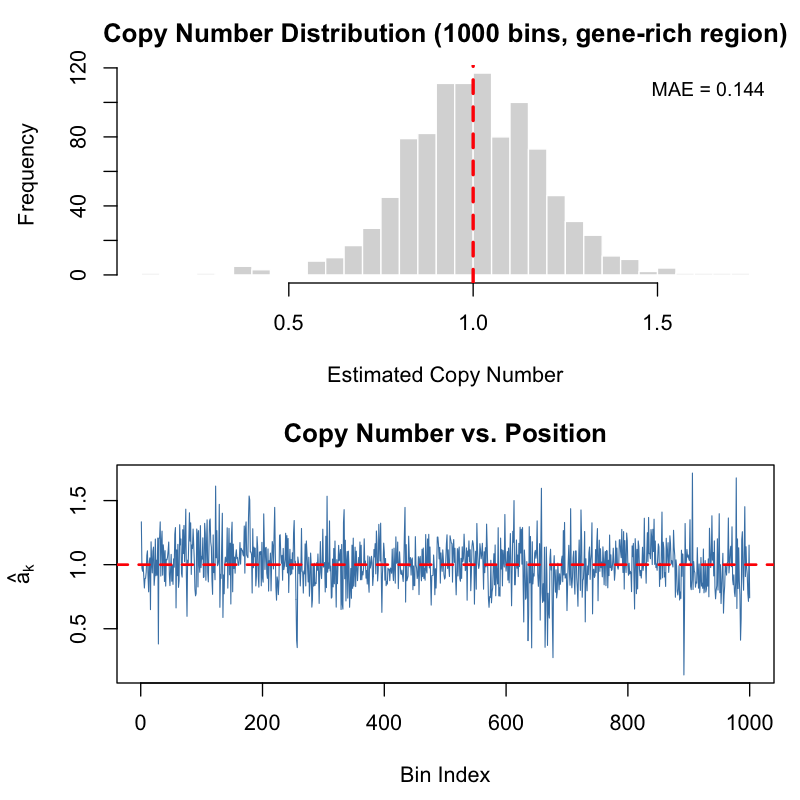
\includegraphics[width=0.75\textwidth]{fig_lab6_cn}
  \caption{\textbf{Lab 6 --- Copy-number estimates, healthy sample (61.25--63.75 Mb).}
  \textit{Top:} Marginal distribution of $\hat a_k$ across 1000 bins. The histogram is
  centered at 1 (dashed red line), confirming successful GC-bias removal. MAE $\approx 0.15$.
  \textit{Bottom:} Spatial plot of $\hat a_k$ vs.\ bin index. Estimates fluctuate around
  1 without systematic trends, consistent with normal copy number in this region.}
  \label{fig:cn}
\end{figure}

\subsection{Lab 7 --- Tumor vs.\ healthy and aggregative bin-size selection}

\begin{figure}[H]
  \centering
  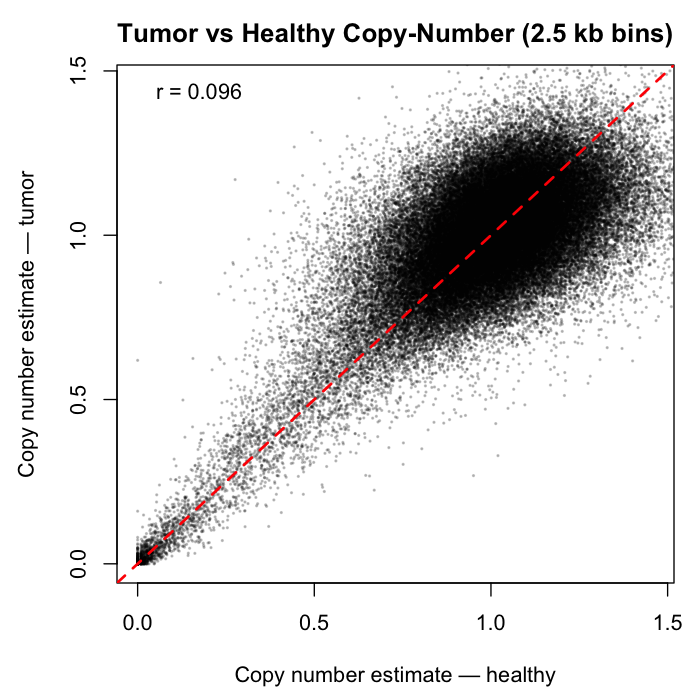
\includegraphics[width=0.60\textwidth]{fig_lab7_scatter}
  \caption{\textbf{Lab 7 Q1 --- Tumor vs.\ healthy copy-number scatter (2.5 kb bins).}
  Each point is one genomic bin. The correlation is very weak ($r=0.096$), reflecting
  tumor-specific CN changes plus substantial bin-level noise at 2.5 kb resolution.
  The red diagonal is the line of equality. Both samples are normalized to median = 1.}
  \label{fig:tumor_scatter}
\end{figure}

\textbf{Q1 --- Paired comparison.} Healthy and tumor samples (\code{lib2}), 2500-bp bins,
two chromosome arms (A: 5--119.99~Mb, B: 130--242~Mb; lengths chosen as multiples of
10~kb so all bin sizes align). Separate GC splines per sample ($R^2$: healthy
\textbf{0.629}, tumor \textbf{0.484}; the tumor curve is less stable at GC extremes,
reflecting greater heterogeneity). After per-sample median-normalized correction, the
bin-level tumor-vs-healthy CN correlation is \textbf{$r\approx 0.10$}
(Figure~\ref{fig:tumor_scatter}) --- tumor-specific CN changes plus 2.5-kb bin noise.

\begin{figure}[H]
  \centering
  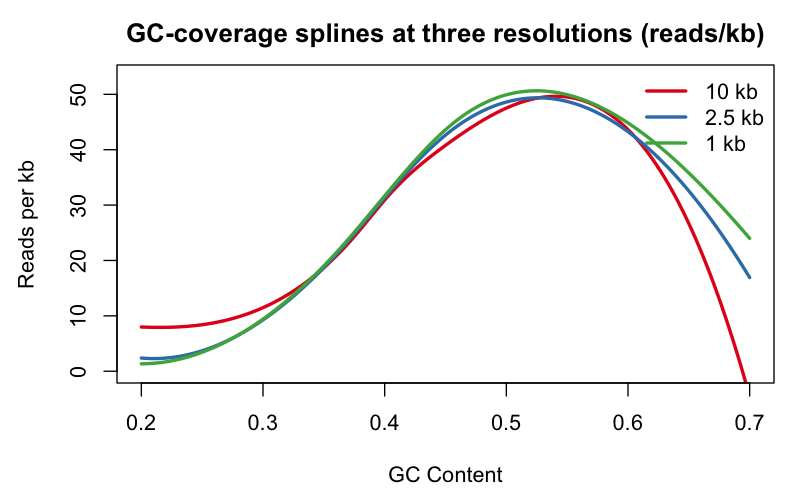
\includegraphics[width=0.85\textwidth]{fig_lab7_splines}
  \caption{\textbf{Lab 7 Q2 --- GC--coverage splines at three resolutions (reads/kb).}
  Red: 10 kb model; blue: 2.5 kb; green: 1 kb. All three follow the same qualitative
  unimodal shape. Differences are largest in the low- and high-GC tails (extrapolation),
  where data are sparse. Expressing predictions in reads/kb removes the trivial bin-size
  scaling and reveals the residual shape differences.}
  \label{fig:splines_q2}
\end{figure}

\textbf{Q2 --- Aggregative model.} GC splines fit at three resolutions (10k / 2.5k / 1k),
with held-out 10-kb test cells predicted either directly or by summing 4/10 sub-cell
predictions (Figure~\ref{fig:splines_q2}). Model selection followed the lab-4 candidate
set (4 knot/degree variants), 80/20 fit/val split, \code{set.seed(22)}. \textbf{1~kb
gives the best held-out test loss}: smaller bins retain local GC structure that lets the
spline track the true coverage profile more accurately, and the summing step aggregates
those fine predictions back to the 10-kb scale without discarding that information.
This is the bias--variance tradeoff in action: larger bins cut per-bin noise but blur
the local GC signal; the aggregative approach captures the best of both.

% ==================================================================
\subsection{Lab 9 --- Anomaly detection: CNV calling on the two-sample data}

Lab 9 brought together all the earlier machinery to ask: \emph{which genomic bins show a
statistically significant tumor-specific copy-number change?} The workflow has four stages.

\paragraph{Test statistic (Part A).}
We work with the two-sample GC-corrected ratio
$\hat a_k = \hat a^\text{tumor}_k / \hat a^\text{healthy}_k$, where each sample is
corrected by its own GC spline and median-normalized (the lab-8 method). Dividing
cancels shared GC bias and library-specific technical effects, leaving a cleaner CN
signal. The statistic is
\[
  S1_k = \log_2(\hat a_k).
\]
Under $H_0$ (no tumor-specific CN change, ratio = 1) this is centered at 0; gains are
positive, losses negative; the $\log_2$ scale is natural (value 1 = doubling,
$-1$ = halving). We also evaluated robust window aggregates (trimmed mean S2, Huber
M-estimator S3) but found them unnecessary once the negative control filter is applied
(see below).

\paragraph{Negative controls and the empirical null (Part B).}
We need a direct sample from the distribution of $S1$ when $H_0$ is true. We apply a
\textbf{local stability filter}: a bin is kept as a negative control only if its
11-bin neighbourhood has both a median near zero ($|\tilde T| \leq \log_2 1.10$) and
low scatter ($\text{SD} \leq \log_2 1.15$). Filtering on the two-sample \emph{ratio}
(not the healthy sample alone) is correct: $H_0$ is ``no tumor-specific change'', so
germline CNVs shared by both samples correctly pass the filter. About 37\% of non-zero
bins pass ($\sim$31,000 controls), giving an empirical null resolving p-values down to
$\approx 3\times 10^{-5}$.

Calibration was verified by a split-half check (interleaved 100-bin blocks so null and
test bins never share a window). S1 tracked the uniform diagonal almost perfectly
(KS $D\approx 0.009$; Figure~\ref{fig:calibration}). S2/S3 were slightly conservative
(over-compression caused by redundant aggregation), costing power with no compensating
gain, so S1 was carried forward.

\begin{figure}[H]
  \centering
  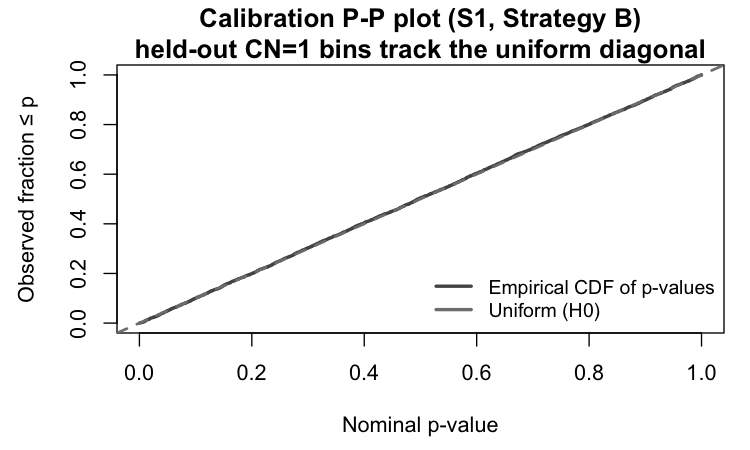
\includegraphics[width=0.68\textwidth]{fig_lab9_calibration}
  \caption{\textbf{Lab 9 --- Calibration P-P plot.}
  Empirical CDF of held-out CN=1 bin p-values vs.\ the uniform diagonal.
  S1 tracks the diagonal closely, confirming the empirical null is well-calibrated:
  the realised false-positive rate matches the nominal $\alpha$ at every level.}
  \label{fig:calibration}
\end{figure}

\paragraph{P-values and multiple testing (Parts C--D).}
For each testable bin the two-sided empirical p-value is
\[
  p_k = \frac{\bigl|\{j \in \text{ctrl} : |S1_j| \geq |S1_k|\}\bigr|}{|\text{ctrl}|}.
\]
Comparing empirical vs.\ parametric (Normal) p-values: the two methods agree on the
$\sim$2,340 most extreme bins; the empirical test keeps 573 additional marginal bins
that the Normal model drops, while the parametric assigns single-bin p-values as small
as $10^{-133}$ --- a precision the 31,000 control observations cannot support.

\textbf{Multiple testing.} With $\sim$85,000 bins tested, Bonferroni would collapse the
per-test threshold to $\approx 10^{-7}$ and eliminate almost all true events.
We use the \textbf{Benjamini--Hochberg (BH) procedure} instead, which controls the
\textbf{False Discovery Rate} (FDR): the expected proportion of false positives
\emph{among the significant calls}, not the probability of any single false call.
At FDR target 0.01, adjacent significant bins are grouped by run-length encoding
(\code{rle}) into continuous segments.

\paragraph{Results (Parts D--F).}
Figure~\ref{fig:cnv} shows the genome-wide result. After BH correction at FDR~$<0.01$:
\begin{itemize}[leftmargin=*]
  \item \textbf{1,600 gain bins} and \textbf{1,313 loss bins}.
  \item Clearest focal \textbf{deletion near 28.5 Mb} (mean ratio $\approx 0.54$,
    roughly a two-fold loss).
  \item \textbf{Cluster of losses at $\sim$141--142 Mb} (post-centromere).
  \item The centromere gap (120--130 Mb) is untested, not mis-called as a loss.
\end{itemize}

\begin{figure}[H]
  \centering
  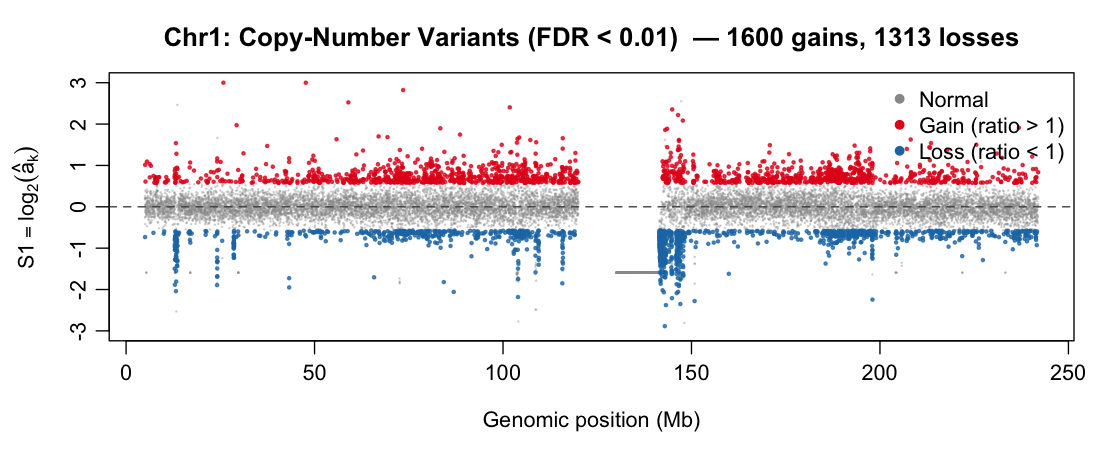
\includegraphics[width=\textwidth]{fig_lab9_cnv}
  \caption{\textbf{Lab 9 --- Genome-wide copy-number variants, chr1.}
  Each point is one 2.5 kb bin. Grey: not significant. Red: gain ($\hat a > 1$).
  Blue: loss ($\hat a < 1$). The centromere gap ($\sim$120--130 Mb) is left untested
  (bins with zero coverage in either sample are excluded). The clearest loss cluster
  is near 28.5 Mb; gains are more scattered.}
  \label{fig:cnv}
\end{figure}

% ==================================================================
\section{Key Numbers}
% ==================================================================

\begin{center}
\begin{tabular}{@{}lll@{}}
\toprule
\textbf{Quantity} & \textbf{Value} & \textbf{Lab} \\
\midrule
Base-level mean coverage $\lambda$ (50--60 Mb) & $\approx 0.036$ reads/base & 3 \\
Binned VMR (uniform-Poisson test)              & $\approx 14.7$             & 3 \\
GC--coverage Pearson correlation $r$           & $\approx 0.84$             & 3 \\
Spline $R^2$ ceiling (50--100 Mb, 5 kb)        & $\approx 0.75$             & 4 \\
Residual SD ratio (high/low GC quartile)       & $\approx 2.25$             & 4 \\
$R^2$ gain from $G{+}C$ vs.\ single base        & $\approx 0.17$             & 5 \\
Quasi-Poisson dispersion $\phi$ (after GC)     & $\approx 14$               & 5 \\
Copy-number MAE from baseline                  & $\approx 0.15$             & 6 \\
Variance split (Poisson / $\epsilon$)          & $\approx 16\%$ / $84\%$    & 6 \\
Total $\mathrm{Var}(\hat a_k)$                  & $\approx 0.09$             & 6 \\
GC spline $R^2$ (healthy / tumor)              & $0.629$ / $0.484$          & 7 \\
Tumor vs.\ healthy CN correlation $r$          & $\approx 0.10$             & 7 \\
\midrule
Negative control bins (Strategy B)             & $\sim$31,000 (37\% of nz)  & 9 \\
Calibration KS $D$ (S1, split-half)            & $\approx 0.009$            & 9 \\
Significant gain bins after BH (FDR $<0.01$)   & 1,600                      & 9 \\
Significant loss bins after BH (FDR $<0.01$)   & 1,313                      & 9 \\
Focal deletion                                 & $\sim$28.5 Mb, ratio $\approx 0.54$ & 9 \\
\midrule
High-GC anomaly region                         & cells 3000--5500 ($\sim$53--55.5 Mb) & 1 \\
Centromere gap                                 & $\sim$120--130 Mb          & 2 \\
Statistical elbow for bin size                 & $\sim$5 kb                 & 5 \\
Default model region                           & 50--100 Mb                 & 3--7 \\
Default bin size (labs 3--5)                   & 5000 bp                    & 3--5 \\
Default bin size (labs 6--7)                   & 2500 bp                    & 6--7 \\
\bottomrule
\end{tabular}
\end{center}

% ==================================================================
\section{Methods and Tools Reference}
% ==================================================================

\textbf{Statistical methods covered:}
base-composition EDA; coverage binning; the uniform Poisson model and its three
assumptions; VMR and the variance decomposition for overdispersion; linear regression
(\code{lm}) with residual diagnostics; cubic / B-spline non-parametric regression
(\code{bs}); knot/degree model selection; train/validation/test splits, learning
curves, and the bias--variance tradeoff; Poisson and quasi-Poisson GLMs (log link)
with dispersion parameter $\phi$; the plug-in copy-number estimator with median
normalization; bias and variance of the estimator; additive vs.\ multiplicative noise;
two-sample comparison.

\textbf{R toolkit:}
\code{data.table::fread} (fast I/O), \code{tabulate} (fast coverage counting),
\code{tictoc} (benchmarking), base graphics throughout with colorblind-friendly palette
(\code{\#56B4E9}/\code{\#E69F00}), transparent points, running medians via \code{runmed()},
\code{splines::bs}, \code{glm}, \code{kableExtra}, \code{shiny} (interactive GC explorer,
Lab 5). Shared code in \code{utils.R} (coverage counting) and \code{lab5\_utils.R}
(binning, spline fitting, plotting, metrics, \code{fit\_gc\_spline()}).

\textbf{Foundational reference:}
Y.~Benjamini and T.~P.~Speed (2012), ``Summarizing and correcting the GC content bias
in high-throughput sequencing,'' \textit{Nucleic Acids Research} \textbf{40}(10):e72.
This paper supplies the central phenomenon (GC bias is unimodal, fragment-level,
PCR-driven), the coverage-as-$a_k\,f(\text{gc}_k)$ decomposition, and the
correction-by-normalization strategy that the entire lab series implements step by step.

\end{document}
